% Created 2024-11-10 Sun 23:01
% Intended LaTeX compiler: pdflatex
\documentclass[11pt]{article}
\usepackage[utf8]{inputenc}
\usepackage[T1]{fontenc}
\usepackage{graphicx}
\usepackage{longtable}
\usepackage{wrapfig}
\usepackage{rotating}
\usepackage[normalem]{ulem}
\usepackage{amsmath}
\usepackage{amssymb}
\usepackage{capt-of}
\usepackage{hyperref}
\usepackage{parskip,darkmode}
\enabledarkmode
\usepackage{tikz,xcolor}
\usetikzlibrary{shapes.geometric, arrows, positioning}
\author{DESKTOP-H800RKQ}
\date{\today}
\title{Inference And Sampling}
\hypersetup{
 pdfauthor={DESKTOP-H800RKQ},
 pdftitle={Inference And Sampling},
 pdfkeywords={},
 pdfsubject={},
 pdfcreator={Emacs 29.4 (Org mode 9.7.11)}, 
 pdflang={English}}
\begin{document}

\maketitle
\tableofcontents

\section{Hidden Markov Models}
\label{sec:org05978cf}
A node may repeat over time, so this requires an explicit encoding of time.
A chain has a length equal to the amount of time modeled.
Times can be \textbf{event-driven} or \textbf{clock-driven}.

The \textbf{Markov assumption}
$$ P(S_{t+1} \mid S_{1}, \dots, S_{t}) = P(S_{t+1} \mid S_{t}) $$
gives the dynamics of the Markov chain.

In a \textbf{Hidden Markov Model (HMM)} observations \(O_{t}\) and observation
functions \(P(O_{t} \mid S_{t})\) are added to the states.
The observations are always observed, so their nodes are square.

\begin{center}
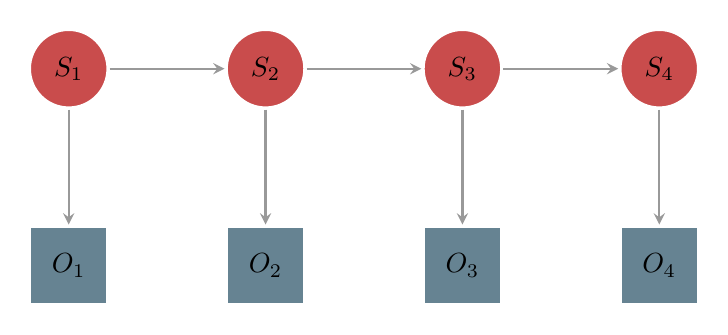
\begin{tikzpicture}[node distance=2.5cm]

\definecolor{arrowcolor}{rgb}{0.6, 0.6, 0.6}

\tikzstyle{state} = [circle, draw=white, fill=red!70!black!70, very thick, minimum size=1cm]
\tikzstyle{obs} = [rectangle, draw=white, fill=cyan!40!black!80, very thick, minimum size=1cm]
\tikzstyle{arrow} = [->, thick, draw=arrowcolor, >=stealth]

\node[state] (S1) {$S_{1}$};
\node[state, right of=S1] (S2) {$S_{2}$};
\node[state, right of=S2] (S3) {$S_{3}$};
\node[state, right of=S3] (S4) {$S_{4}$};

\node[obs, below of=S1] (O1) {$O_{1}$};
\node[obs, below of=S2] (O2) {$O_{2}$};
\node[obs, below of=S3] (O3) {$O_{3}$};
\node[obs, below of=S4] (O4) {$O_{4}$};

\draw[arrow] (S1) -- (S2) node[midway, right] {};
\draw[arrow] (S2) -- (S3) node[midway, right] {};
\draw[arrow] (S3) -- (S4) node[midway, right] {};

\draw[arrow] (S1) -- (O1) node[midway, above] {};
\draw[arrow] (S2) -- (O2) node[midway, above] {};
\draw[arrow] (S3) -- (O3) node[midway, above] {};
\draw[arrow] (S4) -- (O4) node[midway, above] {};

\end{tikzpicture}
\end{center}

Given a sequence of observations \(O_{1}, \dots, O_{t}\), the following
can be estimated:
$$ P(S_{t} \mid O_{1}, \dots, O_{t}) $$
and
$$ P(S_{k} \mid O_{1}, \dots, O_{k}) \; \text{for $k < t$} $$

The most well-known application of HMMs is in speech recognition.
These can be built in a hierarchical model, with higher-level models
having words as states to built sentences as HMMs and lower-level
models having phonemes as states to have words as HMMs.
Observations are generally audio features, with different
levels of granularity of audio features being present in different
levels of models.
\subsection{Belief Monitoring}
\label{sec:org327feb1}
\subsubsection{Forward}
\label{sec:orgaefdfe1}
$$ \alpha_{t} (i) = P(O_{1 \dots t}, S_{t} = i) = P(O_{t} \mid S_{t} = i) \sum_{S_{t-1}} P(S_{t} = i \mid s_{t-1}) \alpha_{t-1}(s_{t-1}) $$
\subsubsection{Backward}
\label{sec:orgb9a8482}
$$ \beta_{t}(i) = P(O_{t+1 \dots T} \mid S_{t} = i) = \sum_{s_{t+1}} \beta_{t+1} (s_{t+1}) P(O_{t+1} \mid s_{t+1}) P(s_{t+1} \mid S_{t} = i) $$
\subsubsection{Forward-Backward}
\label{sec:org467dcf4}
$$ \alpha_{t}(i) \beta_{t}(i) = P(O_{1 \dots T}, S_{t} = i) \propto P(S_{t} = i \mid O) $$
\section{Dynamic Bayesian Networks}
\label{sec:org451e7f7}
Any Bayesian network can repeat over time, which is a \textbf{Dynamic Bayesian Network}.
Many examples can be solved with variable elimination though they can become too complex with
enough variables.

Bayesian probability ensures that evidence is integrated proportionally to its precision,
so sensors are \textbf{precision weighted}.

Variable elimination is an exact algorithm, and sometimes these calculations can be difficult
or probability distributions are unknown.
This requires resorting to stochastic sampling, since sampling from a distribution allows
for estimation.
\section{Sampling}
\label{sec:org544a756}
With \textbf{stochastic simulation}, get probabilities from samples.
Specifically, sample from a variable's posterior probability to estimate its posterior
probability.

To generate samples from a distribution for a variable \(X\) with a discrete domain or a real
domain:
\begin{itemize}
\item totally order values of the domain of \(X\)
\item generate the cumulative probability distribution \(f(x) = P(X \le x)\)
\item select a value \(y\) uniformly in the range \([0, 1]\)
\item select the \(x\) such that \(f(x) = y\)
\end{itemize}
\subsection{Forward Sampling}
\label{sec:org7b18bf8}
Sample variables one at a time, specifically sampling parents before sampling a node.
Given values for the parents of \(X\), sample from the probability of \(X\) given its parents.

For samples \(s_{i}\), \(i = 1 \dots N\)
$$ P(X = x_{i}) \propto \sum_{s_{i}} \delta (x_{i}) = N_{X=x_{i}} $$
where \(\delta(x_{i})\) is 1 if \(X = x_{i}\) in \(s_{i}\) and 0 otherwise.

Inference via sampling approaches the probability as the number of samples increases.
\end{document}
